\PassOptionsToPackage{xetex}{xcolor}
\PassOptionsToPackage{xetex}{graphicx}
\documentclass[a4paper,landscape,headrule,footrule,xetex,25pt]{foils}

\input{headx.tex}

\begin{document}
\header{}{Introduction, Organization}{What does it mean to mean?}
\maketitle

%\include{schedule}



\myslide{Welcome!}

\begin{itemize}
\item In this course we will introduce you to the study of meaning
  \begin{itemize}
  \item How meaning is built up from words and phrases
  \item How meaning depends on context
  \end{itemize}
\item We will ground the analysis with real examples from the Sherlock Holmes stories and the War with the Newts
  \begin{itemize}
  \item I try to make this as enjoyable as possible
  \item You get to read  a great story
  \end{itemize}
\end{itemize}


\myslide{Overview of today}

\begin{itemize}
\item How this course is organized
\item What is \txx{semantics} (and \txx{pragmatics})
\item Why should we be interested in semantics
\item Ways of looking at the world (\txx{Views})
\item Words that change meaning when you use them! (\txx{Deixis})
\item Syllabus; Administrivia
\end{itemize}




\myslide{Textbook and Readings}

\begin{itemize}
\item No required text book and not much reading
\item \emp{EXCEPT you must read the story assigned}
\item If you want to know more about semantics I recommend
  \begin{itemize}
  \item Paul Kroeger (2022) \textit{Analyzing meaning: An introduction to semantics and pragmatics}. 3rd edition.  Language Science Press. \href{https://langsci-press.org/catalog/book/359}{DOI: 10.5281}
  \item Saeed, John (2009) \textit{Semantics}. 4rd Edition. Wiley-Blackwell. 
  \item Lyons, John (1977) \textit{Semantics}.  Cambridge University Press
  \end{itemize}
\item Between now and next week, I expect you to read the first chapter of the assigned story.
\end{itemize}

\myslide{Studying meaning}

\begin{itemize}
\item You'll learn to analyze meaning systematically, using examples from the \textit{War with the Newts}
  \begin{itemize}
  \item Word Meaning (sense)
%    \\   https://compling.upol.cz/ntumc/cgi-bin/showcorpus.cgi
    \\  \eng{to knock up}
  \item Word and Sentence Meaning (sentiment)
    \\  \eng{Julia and I had no great pleasure in our lives}
  \item Idioms and metaphors
    \\ \eng{to cross someone's path}
  \end{itemize}
% \item You must do the three online projects, each is 4--6 hours work

\end{itemize}



% Other References

% Biber, D., S. Conrad \& R. Reppen, Corpus Linguistics: Investigating Language Structure and Use. Cambridge University Press, 1998.

% Kennedy, G. An Introduction to Corpus Linguistics. Longman, 1998.

% McEnery, Tony et al. Corpus-Based Language Studies: An Advanced Resource Book. Routledge, 2006.

% McEnery, Tony and Andrew Wilson Corpus Linguistics 2nd ed, Edinburgh UP, 2001

% Sinclair, John. Corpus Concordance Collocation. Oxford: Oxford UP, 1991



\section{Introduction to Semantics}

\myslide{What is Semantics}
\begin{itemize}
\item Very broadly, semantics is the study of meaning
  \begin{itemize}
  \item Word meaning
  \item Sentence meaning
  \end{itemize}
\item Why do we want to study meaning?
\item What kind of knowledge does it take for a speaker to produce language and for a hearer to comprehend language? 
\end{itemize}

\myslide{Layers of Linguistic Analysis}
\begin{enumerate}\addtolength{\itemsep}{-0.75ex}
\item Phonetics \& Phonology
\item Morphology
\item Syntax
\item \txx{Semantics}
\item \txx{Pragmatics}
\item Stylistics
\end{enumerate}
% Two theories
% \begin{itemize}
% \item Semantics is \txx{autonomous}, a separate module
% \item Semantics is \txx{integrated} with other knowledge, inseparable
%   \begin{itemize}
%   \item linguistic knowledge is inseparable from encyclopedic knowledge
%   \end{itemize}
% \end{itemize}

\myslide{Do people share a common conceptual system?}

\begin{itemize}
\item What is a \lex{high school}?
\item What color is \lex{blue}?
\item What does \lex{verb} mean?
\item What is  \lex{carrot cake}?
\end{itemize}

\newpage

Japanese traffic lights are green (as required by international
agreements).  However they are typically called 青い \jpn[blue]{aoi},
the same word as the color of the sky.  Historically this color
historically covered both green and blue ``grue'',
with 緑 \jpn[green]{midori} being a later addition.  For this reason,
the Japanese government decided in 1973 to change the color of the go
light to the bluest possible hue of green!


\href{https://www.japantimes.co.jp/life/2013/02/25/language/the-japanese-traffic-light-blues-stop-on-red-go-on-what/#.WRmAuuWGNPZ}{The Japanese traffic light blues: Stop on red, go on what?}
 

\myslide{Word Meaning and Sentence Meaning}

\begin{itemize}
\item We store information about words in our \txx{mental lexicon}
  \begin{itemize}
  \item It is still unclear what exactly a word is!
  \end{itemize}
\item Words can be combined to form an infinite number of expressions
  \begin{itemize}
  \item This building up of meaning is referred to as \txx{composition}
  \item If the meaning of the whole can be deduced from the parts then it is \txx{compositional}
  \end{itemize}
\end{itemize}

\myslide{Reference and Sense}

\begin{itemize}
\item Words \txx{refer} to things in the world (like \iz{unicorn}s)
\item The meaning of a word across different contexts is often referred to as its \txx{sense}
  \begin{itemize}
  \item Same word can refer to different things
    \begin{itemize}
    \item English: \eng{I put my money in the \ul{bank}}
    \item English: \eng{I fell asleep at the river \ul{bank}}
    \end{itemize}
  \item Same basic concept can have different boundaries
    \begin{itemize}
    \item French: \eng[sheep/mutton]{mouton}
    \item English: \eng{sheep} vs \eng{mutton}
      
    \item Japanese: \eng[dove/pigeon]{hato}
    \item English: \eng{dove} vs \eng{pigeon}
    \end{itemize}
  \end{itemize}
\end{itemize}




\myslide{Representing meaning}
\MyLogo{Also vector space, description, images, video, \ldots}
\begin{itemize}
\item One of our goals will be to represent meaning
\item There are various ways to do this
  \begin{itemize}
  \item Syntactic trees
  \item Logical forms
  \item Thesauri and Ontologies 
  \item Translation
  \item Paraphrasing
  \end{itemize}
Can you think of others?

\item At the end of this course you should be able to use these to
  describe many aspects of meaning
\end{itemize}



\myslide{Language is normally under-specified}
\MyLogo{There are many meanings}
\begin{center}
\large We get \blu{words}: \\[2ex]
    \Large \eng{I saw a kid with a cat.} \\[3ex]
We want \emp{meaning}:
\\  \includegraphics[width=0.3\textwidth]{pics/1.png}
\end{center}



\myslide{I saw a kid with a cat$_1$}
\MyLogo{Thanks to Eddy and Zina Pozen for the pictures}

\hspace{-3em}\begin{tabular}{ll}

  \includegraphics[width=0.5\textwidth]{pics/1.png}
&
  \begin{minipage}{0.45\textwidth}
    \vspace*{-8ex}
\begin{scriptsize}
 {%
 \leaf{\emph{I}}
 \branch{1}{NP}
 \leaf{\emph{saw}}
 \branch{1}{V:see}
 \leaf{\emph{a}}
 \branch{1}{DET}
 \leaf{\emph{kid}}
 \branch{1}{N}
 \leaf{\emph{with a cat}}
\branch{1}{PP[together]}
%\branch{2}{\ibar{N}}
\branch{3}{NP}
 \branch{2}{VP}
 \branch{2}{S}
 \qobitree}
\end{scriptsize}
\\[3ex]
 \small \iz{see(I, kid: \textsc{past});  with(kid, cat)}
\\[1ex] \iz{see $\subset$ perceive}
\\ \iz{kid $\sim$ child}
\\ \iz{with $\subset$ together}
\end{minipage}

\end{tabular}

\myslide{I saw a kid with a cat$_2$}
\MyLogo{}
\hspace{-3em}\begin{tabular}{ll}
  \includegraphics[width=0.5\textwidth]{pics/2.png}
&
  \begin{minipage}{0.45\textwidth}
    \vspace*{-10ex}
\begin{scriptsize}
 {%
 \leaf{\emph{I}}
 \branch{1}{NP}
 \leaf{\emph{saw}}
 \branch{1}{V:see}
 \leaf{\emph{a}}
 \branch{1}{DET}
 \leaf{\emph{kid}}
 \branch{1}{N}
\branch{2}{NP}
 \leaf{\emph{with a cat}}
\branch{1}{PP[together]}
 \branch{3}{VP}
 \branch{2}{S}
 \qobitree}
\end{scriptsize}
\\[3ex]
 \small 
 \iz{see(I, kid: \textsc{past}) with(I, cat)}
\\[1ex] \iz{see $\subset$ perceive}
\\ \iz{kid $\sim$ child}
\\ \iz{with $\subset$ together}
\end{minipage}
\end{tabular}




\myslide{I saw a kid with a cat$_3$}
\hspace{-3em}\begin{tabular}{ll}
  \includegraphics[width=0.5\textwidth]{pics/3.png}

&
  \begin{minipage}{0.45\textwidth}
    \vspace*{-20ex}
\begin{scriptsize}
 {%
 \leaf{\emph{I}}
 \branch{1}{NP}
 \leaf{\emph{saw}}
 \branch{1}{V:saw}
 \leaf{\emph{a}}
 \branch{1}{DET}
 \leaf{\emph{kid}}
 \branch{1}{N}
 \leaf{\emph{with a cat}}
\branch{1}{PP[together]}
%\branch{2}{\ibar{N}}
\branch{3}{NP}
 \branch{2}{VP}
 \branch{2}{S}
 \qobitree}
\end{scriptsize}
\\[3ex]
 \small 
\iz{saw(I, kid: \textsc{pres});  with(kid, cat)}
\\[1ex] \iz{saw $\subset$ cut}
\\ \iz{kid $\sim$ child}
\\ \iz{with $\subset$ together}
\end{minipage}
\end{tabular}



\myslide{I saw a kid with a cat$_4$}
\hspace{-3em}\begin{tabular}{ll}
  \includegraphics[width=0.5\textwidth]{pics/4.png}
&
  \begin{minipage}{0.45\textwidth}
    \vspace*{-20ex}
\begin{scriptsize}
 {%
 \leaf{\emph{I}}
 \branch{1}{NP}
 \leaf{\emph{saw}}
 \branch{1}{V:saw}
 \leaf{\emph{a}}
 \branch{1}{DET}
 \leaf{\makebox[1em]{\emph{kid} [goat]}}
 \branch{1}{N}
\branch{2}{NP}
 \leaf{\emph{with a cat}}
\branch{1}{PP[together]}
 \branch{3}{VP}
 \branch{2}{S}
 \qobitree}
\end{scriptsize}
\\[3ex]
 \small 
\iz{saw(I, kid: \textsc{present}) with(I, cat)}
\\[1ex] \iz{saw $\subset$ cut}
\\ \iz{kid $\sim$ young goat}
\\ \iz{with $\subset$ together}
\end{minipage}
\end{tabular}


\myslide{I saw a kid with a cat$_5$}
\hspace{-3em}\begin{tabular}{ll}
  \includegraphics[width=0.5\textwidth]{pics/5.png}
&
  \begin{minipage}{0.45\textwidth}
    \vspace*{-20ex}
\begin{scriptsize}
 {%
 \leaf{\emph{I}}
 \branch{1}{NP}
 \leaf{\emph{saw}}
 \branch{1}{V:see}
 \leaf{\emph{a}}
 \branch{1}{DET}
 \leaf{\emph{kid}}
 \branch{1}{N}
\branch{2}{NP}
 \leaf{\emph{with a cat}}
\branch{1}{PP[instrument]}
 \branch{3}{VP}
 \branch{2}{S}
 \qobitree}
\end{scriptsize}
\\[3ex]
 \small 
 \iz{see(I, kid: \textsc{past}) with(I, cat) }
\\[1ex] \iz{see $\subset$ perceive}
\\ \iz{kid $\sim$ child}
\\ \iz{with $\subset$ instrumental}
 \end{minipage}
\end{tabular}


% \myslide{People are good at understanding}
% \MyLogo{We do this too}
% \begin{itemize}
% \item The words only hint at the meaning
% \item Many words can mean more than one thing (\blu{ambiguity})
% \item How can we \blu{model} and \blu{resolve} ambiguity?
% \item Look at the text and try to annotate the meaning
%   \begin{center}
%     Very hard work
%   \end{center}
% %   \begin{itemize}
% %   \item Deduce implicit models
% %     \begin{itemize}
% %     \item bag of words, $n$-gram chunks, \ldots
% %     \end{itemize}
% %   \item Define explicit models
% %     \begin{itemize}
% %     \item Grammars, lexicons and thesauri
% %     \end{itemize}
% %   \end{itemize}
% %\item Then build statistical language models (machine learning)
% \end{itemize}

\myslide{We can also use translations}
%\MyLogo{Work smarter}
%\addtocounter{exx}{-13}
\begin{exe}
  \ex \glll 我 看到了 一个 抱着 猫 的 孩子 \\
  wǒ   kàndàole    yīgè   bàozhe  māo  de    háizi. \\
  I saw one holding cat 's child \\
  \trans I did see a child holding a cat

  \ex \glll 我 抱着 猫 看到了 一个 孩子 \\
  wǒ  bàozhe māo kàndàole  yīgè     háizi \\
  I holding cat saw one  child \\
 \trans I holding a cat did see a child
%鋸锯
  \ex \glll 我 鋸  一个 孩子 和 他/她 的 猫 \\
wǒ jù  yīgè    háizi  hé  tā/tā   de māo \\
%wo3 ju4  yi1ge4    háizi  he2  ta1ta1   de ma1o\\
 I      saw    one    child   and     he/she  's cat\\
 \trans I saw  (cut with a saw) a child and their cat 

  \ex \glll 我 和 一只 猫 鋸 一只 小 山羊 \\
wǒ hē  yīzhǐ  māo jù yīzhǐ xiǎo  shānyáng  \\
%wo3 he1  yi1zhi3  ma1o ju4 yi1zhi3 xia3o  sha1nya2ng    \\
I and one cat saw (cut with a saw) one small goat \\

\trans I and a cat saw a young goat
  \ex \glll 我 用 一只 猫 看到了 一个 孩子 \\
wǒ yòng yīzhǐ  māo kàndàole  yīgè  háizi \\
I use one cat saw one child \\
\trans Using a cat, I did see a child
\end{exe}

\bigskip
\begin{center} \large
  Your turn: try to paraphrase --- translate into English
  \\ aim to be unambiguous, even if slightly disfluent\task
\end{center}
\section{Where is the meaning?}

\myslide{Referential or Representational?}

One view of meaning is to define it in terms of how it constrains reality.

\begin{itemize}
\item Picture the worlds in which these sentences are true:
  \begin{exe}
    \ex \eng{I patted the dog.}
    \ex \eng{I did not pat the dog.}
  \end{exe}
\end{itemize}

Assuming that they were uttered at the same time, they are
incompatible because they cannot refer to the same
situation: the \txx{referential} view. 
\newpage
But we can represent the same reality in different ways:

\begin{exe}
  \ex \eng{Ich habe Hunger} ``I have hunger''
  \ex \eng{I am hungry}
\end{exe}

\txx{Representational} theories are interested in how we represent reality,
and how our representations are influenced by conceptual structures
conventionalized in language.


 \myslide{Referential View}

\begin{center}
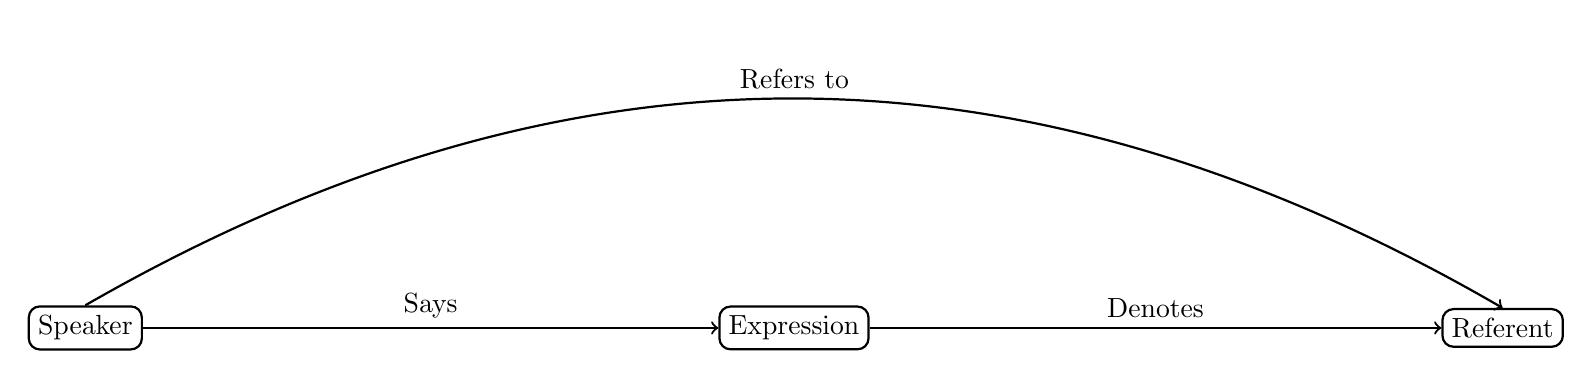
\begin{tikzpicture}[node distance=9cm, auto, thick]
  \node[draw, rounded corners](speaker){Speaker};
  \node[draw, rounded corners, right of=speaker](expression){Expression};
  \node[draw, rounded corners, right of=expression](referent){Referent};

  \draw[->, thick] (speaker) -- node{Says}(expression);
  \draw[->, thick] (expression) -- node{Denotes}(referent);
  \draw[->, thick, bend left] (speaker.north) to node[above]{Refers to}(referent.north);
\end{tikzpicture}
\end{center}


 The \txx{referential view} is focused on direct relationships between
 expressions (words, sentences) and things in the world (realist
 view).





 \myslide{Representational View}

\begin{center}
\begin{tikzpicture}[node distance=8cm, auto, thick]
  \node[draw, rounded corners](speaker){Speaker};
  \node[draw, rounded corners, right of=speaker](expression){Expression};
  \node[draw, rounded corners, above right=1cm and 1.5cm of expression](concept){Concept};
  \node[draw, rounded corners, right of=expression, xshift=3cm](referent){Referent};

  \draw[->, thick] (speaker) -- node{Says}(expression);
  \draw[->, thick] (expression) -- node[left]{Evokes}(concept);
  \draw[->, thick] (concept) -- node[right]{Represents}(referent);
  \draw[->, thick, bend left=30] (speaker) to node[above]{Refers via}(concept);
\end{tikzpicture}
\end{center}

 The \txx{representational view} is focused on how relationships between
 expressions (words, sentences) and things in the world are mediated by
 the mind (cognitive linguistics).  

This gives a more complex, but richer model.


\myslide{Referring vs Non-Referring}

\begin{itemize}
\item \txx{Referring expressions} are expressions that identify
  entities in the world (typically \txx{nominals})
  \begin{exe}
    \ex \eng{cat}, \jpn[that yellow bag]{ano kiiro kaban}
    \ex \eng{London Bridge}, \eng{Xiao Ming}
  \end{exe}
\item \txx{Non-referring expressions} don't have referential properties
  \begin{exe}
    \ex \eng{maybe, if, is, but}
  \end{exe}
\item Not all nominals refer
  \begin{exe}
    \ex \eng{That is \ul{an ugly dog}}
    \ex \eng{If only I had \ul{a dog}}
  \end{exe}
\item And, of course, all this is made more confusing if we model the
  fictional world and our interpretation of it as separate from the
  characters' interpretations, \ldots
\end{itemize}


\section{Deixis}

\myslide{What is Deixis}
\begin{itemize}
\item any linguistic element whose interpretation
  necessarily makes reference to properties of the
  extra-linguistic context in which it occurs is \txx{deictic}
  \begin{description}
  \item[\txx{Person}] relative to the speaker and addressee; \eng{you, me, them}
  \item[\txx{Spatial Location}] demonstratives; \eng{this, that, over there, here}
  \item[\txx{Temporal Location}] tense; \eng{yesterday, today, tomorrow}
  \item[\txx{Social Status}] relative to the social position: \eng{professor, you, uncle, boy}
  \end{description}
\item \txx{Discourse deixis}: referring to a linguistic expression or chunk of discourse
\end{itemize}

\newpage
More than 90\% of the declarative sentences people utter are indexical
in that they involve implicit references to the speaker, addressee,
time and/or place of utterance in expressions like first and second
person pronouns, demonstratives, tenses, and adverbs like \lex{here}, \lex{now},
\lex{yesterday} \citep[p366]{Bar-Hillel:1954}.

\myslide{Spatial Deixis}
\begin{itemize}
\item Two way systems (English, \ldots)
  \\[2ex] \begin{tabular}{llll}
    \txx{proximal} &\lex{this} & \lex{here} &close to the speaker\\
    \txx{distal} &\lex{that} & \lex{there} & far from the speaker 
  \end{tabular}
\item Three (four) way systems (Japanese, \ldots)
    \\[2ex] \begin{tabular}{lllll}
                    & Gloss & \con{thing}   & \con{place}  \\
\hline
      \txx{proximal}  & close to speaker & \lex{kore} ``this'' & \lex{koko} ``here''\\
      \txx{medial} &close to addressee &\lex{sore} ``that''   & \lex{soko} ``there'' \\
      \txx{distal} &far from both&\lex{are} ``\,'tother'' & \lex{asoko} ``over there''  \\ \hline
      \txx{Q} & interrogative & \lex{dore} ``what'' & \lex{doko} ``where''
  \end{tabular}
  \item Can you do English \con{time}?  \task %\marginpar{\fbox{\LARGE ?}}
%  \item Can you do this in another language?\task %\marginpar{\fbox{\LARGE ?}}

 % Can decompose: \lex{here} ``this place'', \lex{there} ``that place'', \lex{where} ``what place''
 % \lex{now} ``this time'',  \lex{then} ``that time'', \lex{when} ``what time''
\end{itemize}

% \noindent\begin{tabular}{lllll}
%     & close to sp  & \multicolumn{2}{c}{far from sp} & Q \\  
%     & & close to hr & far from both \\ \hline
%   English & this & \multicolumn{2}{c}{that} & what \\
%   \ \ \ \  place & here & \multicolumn{2}{c}{there} & where \\
%   Japanese & kono & sono & ano & dono \\
%    \ \ \ \  place & koko & soko & asoko & doko \\
% \end{tabular}


% \mytask{try this}

% \begin{tabular}[l]{}
%   Q & close & far & further \\
%   what & this & that & 'tother \\
%   ?    & now  & then & --- \\
%   where & ? & there & over there \\
% \end{tabular}


\myslide{More Spatial Deixis}

\begin{itemize}
\item Often lexicalized:
  \begin{itemize}
  \item \lex{go, come, foreign, home, local, indigenous, national language}
  \end{itemize}
\item Can lead to \txx{discourse}/\txx{textual deixis}
  \begin{exe}
    \ex \eng{\ul{Here} we begin explaining textual deixis}
  \end{exe}
\item Often also used for time
  \begin{exe}
    \ex \eng{\ul{This year} we are trying a new kind of assignment}
  \end{exe}
\newpage
\item Spatial expressions extend to possession in many languages
  \begin{exe}
    \ex \gll \jpn{NICT-ga} \jpn{Kyoto-ni} \jpn{aru} \\
    NICT-\textsc{nom} Kyoto-\textsc{loc} be \\
    \trans NICT is in Kyoto
    \ex \gll \jpn{watashi-ni} \jpn{musuko-ga}  \jpn{aru} \\
     I-\textsc{loc}  son-\textsc{nom} be \\
    \trans I have a son (lit. a son is in me)
   \end{exe}
\end{itemize}

\myslide{Person Deixis}

\begin{itemize}
\item Minimally a three way division
\\[2ex]  \begin{tabular}{lll}
    First Person & Speaker & \lex{I} \\
    Second Person & Addressee & \lex{you} \\
    Third Person & Other & \lex{he/she/it} \\
  \end{tabular}
\item Often combined with
  \begin{itemize}
  \item \txx{gender}: \lex{he/she/it }
  \item \txx{number}: \lex{I/we}, 
    \lex{'anta} ``you:m'', \lex{'antumaa} ``you:dual'',  \lex{'antum} ``you:m:pl''
    \\ (Arabic)
  \item \txx{inclusion}: \lex{n\'uy} ``we including you'',  \lex{n\'{\i}i} ``we excluding you'' (Zayse)
  \item \txx{honorification}: \lex{kimi} ``you:inferior'', \lex{anata} ``you:equal'',
    \\ don't use pronouns for superiors: \lex{sensei} ``teacher'', \ldots (Japanese)
  \end{itemize}
\end{itemize}

\myslide{Social Deixis}

In European languages, a two-way choice in 2nd person pronominal
reference: the T/V distinction

\begin{itemize}
\item T/V distinctions in European languages
  \\[2ex]
  \begin{tabular}{lll}
    & Familiar 2sg & Polite 2sg \\ \hline
    French & \lex{tu} & \lex{vous} \\
    German & \lex{du} & \lex{Sie} \\
%    Spanish & \lex{t\'u} & \lex{usted} \\
    Czech & \lex{ty} & \lex{vy} \\ 
  \end{tabular}

\item Shift from asymmetric use showing \txx{power} (superior uses \lex{tu}; inferior uses \lex{vous}) to symmetric use showing \txx{solidarity} (strangers use  \lex{vous}; intimates use \lex{tu}): typically the socially superior person must invite the socially
  inferior person to use the familiar form
\end{itemize}

\myslide{Social Deixis can be marked on other words}
\MyLogo{It must be marked}
\begin{exe}
  \ex \jpn{Tanaka-san-ga kudasaimashita} \hfill [addressee and subject hon.]
  \trans Tanaka gave it to me (and I honor him and you)
%  \trans
 \ex \jpn{Tanaka-san-ga kudasatta} \hfill [subject honorification]
  \trans Tanaka gave it to me (and I honor him)

 \ex \jpn{Tanaka-kun-ga kuremashita} \hfill [addressee honorification]
  \trans Tanaka gave it to me (and I honor you)

 \ex \jpn{Tanaka-kun-ga kureta} \hfill [no honorification]
  \trans Tanaka gave it to me (implies I am higher status than him)

\end{exe}

\begin{itemize}
% \item Find examples where someone addresses Sherlock as \eng{Holmes}
%   and compare then to examples where he is addressed as \eng{Mr
%     Holmes}: what is the difference? \task
\item  Find examples in \textit{Válka s Mloky} where \cs{ty} and \cs{vy} are used:  what is the difference? \task
\end{itemize}



\section{Administrivia}

\myslide{Administrivia}
\begin{description}\addtolength{\itemsep}{-5mm}
\item [Coordinator]  Francis \ul{Bond} 
  {\small \url{<bond@ieee.org>}
    \\ ~ \hfill !\url{<francis.bond@upol.cz>}}
\item Details will all be  online:
  \begin{center}
    \url{https://bond-lab.github.io/Semantics/}    
  \end{center}
\end{description}


\myslide{Extra Credit}

\begin{itemize}
\item If you submit a correction that gets accepted for one of the
  resources we use then it shows good mastery of the material
  \begin{itemize}
  \item you can get 1-5\% extra credit (depending on the size/difficulty)
\\ Mark $n \propto 10^{n-1}$ lines of code/documentation
  \item You can't go over 100\%
  \end{itemize}
\item A correction can involve
  \begin{itemize}
  \item fixing an error in transcription or annotation
    \begin{itemize}
    \item spelling error
    \item wrong sense
    \item error in the dictionary
    \end{itemize}
  \item making the documentation easy to read
  \item pointing out an error in a translation / finding a new translation
%  \item  fixing a bug in code
%  \item extending the code with new capabilities
  \end{itemize}

\end{itemize}



\myslide{Student Responsibilities}

By remaining in this class, the student agrees to:
\begin{enumerate}\addtolength{\itemsep}{-1ex}
\item  Make a genuine effort to learn and engage.
\item Read messages and participate.
\item Do assignments on time.
\item Attend regularly.
\item Seek help early, not last minute.
\item Treat peers respectfully.
\end{enumerate}

\myslide{Attendance}
\begin{enumerate}\addtolength{\itemsep}{-1ex}
\item You are expected to attend all classes.
\item Be on time - lateness is disruptive to your own and others' learning.
\item Valid reasons for missing class include the following:
\begin{enumerate}
\item A medical emergency (including mental health emergencies)
\item A family emergency (death, birth, natural disaster, etc).
\end{enumerate}
\item There will be significant material covered in class that is not in your readings.  You cannot expect to do well without coming to class.
\item If you miss a class, it is your responsibility to get the notes, any handouts you missed, schedule changes, etc. from a classmate.
\end{enumerate}

\myslide{Remediation and Academic Integrity}
\begin{enumerate}
\item No late work will be accepted, except in the case of a documented excuse.
\item For planned, justified, absences on class days or days on which assignments are due, advance notice must be provided.
\item Cheating will not be tolerated. Violations, including plagiarism, will be seriously dealt with, and could result in \textbf{a failing grade for the entire course}.
\item Refer to the University Honour Code
\item As always, use your common sense and conscience.
\end{enumerate}


\myslide{Assessment}

\begin{itemize}
\item Participate in tutorials, hand in answers \hfill  20\%
\item Projects 1 \& 2  \hfill 30\% or 25\% (5UJ2)
  \begin{enumerate}
  \item Annotate text individually
  \item Compare annotations and write up result (in groups of four)
  \end{enumerate}
\item Project 3\hfill 5\% (5UJ2)
  \begin{itemize}
  \item Identify interpretations that are not strictly compositional: \\
    idioms and metaphors
  \end{itemize}

\end{itemize}
\hrule
\begin{center}
      You can chose your language and group in moodle \\
      by next Friday \\
      or I will randomly assign you to a language and group
    \end{center}


\myslide{The winning strategy}

\begin{itemize}
\item Read the stories before class (and after again, if necessary)
\item Work together: make study groups
\item Tasks: Discuss as much as you want (but not project 1), annotate your own answers
\item Ask questions \ldots\ early and often!
\end{itemize}


  
\small
\bibliographystyle{aclnat}
\bibliography{abb,mtg,nlp,ling}


% \emp{Next Week}	Theories of meaning and the meaning of words

% \myslide{Acknowledgments and References}
% \MyLogo{If I have seen further, it is by standing on the shoulders of giants (Isaac Newton)}
% \begin{itemize}
% \item Course design and slides inherit from Nala Lee's HG202 course,
%   back in the depths of time (2009).
% \item Thanks to Na-Rae Han for 
%   inspiration for the student policies (from  \textit{LING 2050 Special Topics in Linguistics: Corpus linguistics}, U Penn; adapted).
%   \item Further Reading: 
%   \begin{itemize}
%   \item  Shannon, C.E. (1948), "A Mathematical Theory of Communication", Bell System Technical Journal, 27, pp. 379–423 \& 623–656, July \& October, 1948. \url{http://cm.bell-labs.com/cm/ms/what/shannonday/shannon1948.pdf}
%   \end{itemize}
% \end{itemize}


\myslide{Glossary of Key Terms (English--Czech)}
\begin{flushleft}
\begin{longtable}{ll}
  English & Čestina \\\hline \endhead
Q & otázka (Q) \\
analysis & analýza \\
autonomous & autonomní \\
collocation & kolokace \\
communication & komunikace \\
composition & kompozice \\
compositional & kompoziční \\
concordance & konkordance \\
connotation & konotace \\
context & kontext \\
corpus & korpus \\
deictic & deiktický \\
deixis & deixe \\
denotation & denotace \\
discourse & diskurz \\
distal & distální \\
expression & výraz \\
gender &  (gramatický) rod \\
honorification & honorifika \\
idiom & úsloví \\
inclusion & inkluze \\
lexical & lexikální \\
meaning & význam \\
medial & mediální \\
mental lexicon & mentální lexikon \\
metaphor & metafora \\
nominals & nominální výrazy \\
non-referring expressions & nereferenční výrazy \\
number & číslo \\
person & (gramatická) osoba \\
phrase & slovní spojení \\
power & moc \\
pragmatics & pragmatika \\
proximal & proximální \\
refer & odkazovat \\
reference & reference \\
referential & referenční \\
referential view & referenční pohled \\
referring expressions & referenční výrazy \\
representational & reprezentační \\
representational view & reprezentační pohled \\
semantics & sémantika \\
sense & význam (smysl) \\
sentence meaning & význam věty \\
sentiment & sentiment \\
social status & společenský status \\
solidarity & solidarita \\
spatial location & prostorová lokalizace \\
temporal location & časová lokalizace \\
textual deixis & textová deixe \\
utterance & výpověď \\
word meaning (sense) & slovní význam \\
\end{longtable}
\end{flushleft}

\myslide{Further Reading}

\begin{itemize}
\item Introduction What does it mean to mean?
  \begin{itemize}
  \item Saeed: \S~1
  \end{itemize}

\item Meaning, Thought and Reality
  \begin{itemize}
  \item Saeed: \S~2
  \end{itemize}
  
\item Deixis
  \begin{itemize}
  \item Saeed: \S~7.2
  \end{itemize}
\end{itemize}

\end{document}

%%% Local Variables: 
%%% coding: utf-8
%%% mode: latex
%%% TeX-PDF-mode: t
%%% TeX-engine: xetex
%%% End: 

